\documentclass[1p]{elsarticle_modified}
%\bibliographystyle{elsarticle-num}

%\usepackage[colorlinks]{hyperref}
%\usepackage{abbrmath_seonhwa} %\Abb, \Ascr, \Acal ,\Abf, \Afrak
\usepackage{amsfonts}
\usepackage{amssymb}
\usepackage{amsmath}
\usepackage{amsthm}
\usepackage{scalefnt}
\usepackage{amsbsy}
\usepackage{kotex}
\usepackage{caption}
\usepackage{subfig}
\usepackage{color}
\usepackage{graphicx}
\usepackage{xcolor} %% white, black, red, green, blue, cyan, magenta, yellow
\usepackage{float}
\usepackage{setspace}
\usepackage{hyperref}

\usepackage{tikz}
\usetikzlibrary{arrows}

\usepackage{multirow}
\usepackage{array} % fixed length table
\usepackage{hhline}

%%%%%%%%%%%%%%%%%%%%%
\makeatletter
\renewcommand*\env@matrix[1][\arraystretch]{%
	\edef\arraystretch{#1}%
	\hskip -\arraycolsep
	\let\@ifnextchar\new@ifnextchar
	\array{*\c@MaxMatrixCols c}}
\makeatother %https://tex.stackexchange.com/questions/14071/how-can-i-increase-the-line-spacing-in-a-matrix
%%%%%%%%%%%%%%%

\usepackage[normalem]{ulem}

\newcommand{\msout}[1]{\ifmmode\text{\sout{\ensuremath{#1}}}\else\sout{#1}\fi}
%SOURCE: \msout is \stkout macro in https://tex.stackexchange.com/questions/20609/strikeout-in-math-mode

\newcommand{\cancel}[1]{
	\ifmmode
	{\color{red}\msout{#1}}
	\else
	{\color{red}\sout{#1}}
	\fi
}

\newcommand{\add}[1]{
	{\color{blue}\uwave{#1}}
}

\newcommand{\replace}[2]{
	\ifmmode
	{\color{red}\msout{#1}}{\color{blue}\uwave{#2}}
	\else
	{\color{red}\sout{#1}}{\color{blue}\uwave{#2}}
	\fi
}

\newcommand{\Sol}{\mathcal{S}} %segment
\newcommand{\D}{D} %diagram
\newcommand{\A}{\mathcal{A}} %arc


%%%%%%%%%%%%%%%%%%%%%%%%%%%%%5 test

\def\sl{\operatorname{\textup{SL}}(2,\Cbb)}
\def\psl{\operatorname{\textup{PSL}}(2,\Cbb)}
\def\quan{\mkern 1mu \triangleright \mkern 1mu}

\theoremstyle{definition}
\newtheorem{thm}{Theorem}[section]
\newtheorem{prop}[thm]{Proposition}
\newtheorem{lem}[thm]{Lemma}
\newtheorem{ques}[thm]{Question}
\newtheorem{cor}[thm]{Corollary}
\newtheorem{defn}[thm]{Definition}
\newtheorem{exam}[thm]{Example}
\newtheorem{rmk}[thm]{Remark}
\newtheorem{alg}[thm]{Algorithm}

\newcommand{\I}{\sqrt{-1}}
\begin{document}

%\begin{frontmatter}
%
%\title{Boundary parabolic representations of knots up to 8 crossings}
%
%%% Group authors per affiliation:
%\author{Yunhi Cho} 
%\address{Department of Mathematics, University of Seoul, Seoul, Korea}
%\ead{yhcho@uos.ac.kr}
%
%
%\author{Seonhwa Kim} %\fnref{s_kim}}
%\address{Center for Geometry and Physics, Institute for Basic Science, Pohang, 37673, Korea}
%\ead{ryeona17@ibs.re.kr}
%
%\author{Hyuk Kim}
%\address{Department of Mathematical Sciences, Seoul National University, Seoul 08826, Korea}
%\ead{hyukkim@snu.ac.kr}
%
%\author{Seokbeom Yoon}
%\address{Department of Mathematical Sciences, Seoul National University, Seoul, 08826,  Korea}
%\ead{sbyoon15@snu.ac.kr}
%
%\begin{abstract}
%We find all boundary parabolic representation of knots up to 8 crossings.
%
%\end{abstract}
%\begin{keyword}
%    \MSC[2010] 57M25 
%\end{keyword}
%
%\end{frontmatter}

%\linenumbers
%\tableofcontents
%
\newcommand\colored[1]{\textcolor{white}{\rule[-0.35ex]{0.8em}{1.4ex}}\kern-0.8em\color{red} #1}%
%\newcommand\colored[1]{\textcolor{white}{ #1}\kern-2.17ex	\textcolor{white}{ #1}\kern-1.81ex	\textcolor{white}{ #1}\kern-2.15ex\color{red}#1	}

{\Large $\underline{12n_{0222}~(K12n_{0222})}$}

\setlength{\tabcolsep}{10pt}
\renewcommand{\arraystretch}{1.6}
\vspace{1cm}\begin{tabular}{m{100pt}>{\centering\arraybackslash}m{274pt}}
\multirow{5}{120pt}{
	\centering
	\includegraphics[width=112pt]{../../../GIT/diagram.site/Diagrams/png/2311_12n_0222.png}\\
\ \ \ A knot diagram\footnotemark}&
\allowdisplaybreaks
\textbf{Linearized knot diagam} \\
\cline{2-2}
 &
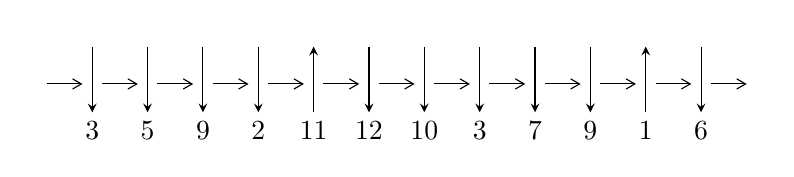
\begin{tikzpicture}[x=20pt, y=17pt]
	% nodes
	\node (C0) at (0, 0) {};
	\node (C1) at (1, 0) {};
	\node (C1U) at (1, +1) {};
	\node (C1D) at (1, -1) {3};

	\node (C2) at (2, 0) {};
	\node (C2U) at (2, +1) {};
	\node (C2D) at (2, -1) {5};

	\node (C3) at (3, 0) {};
	\node (C3U) at (3, +1) {};
	\node (C3D) at (3, -1) {9};

	\node (C4) at (4, 0) {};
	\node (C4U) at (4, +1) {};
	\node (C4D) at (4, -1) {2};

	\node (C5) at (5, 0) {};
	\node (C5U) at (5, +1) {};
	\node (C5D) at (5, -1) {11};

	\node (C6) at (6, 0) {};
	\node (C6U) at (6, +1) {};
	\node (C6D) at (6, -1) {12};

	\node (C7) at (7, 0) {};
	\node (C7U) at (7, +1) {};
	\node (C7D) at (7, -1) {10};

	\node (C8) at (8, 0) {};
	\node (C8U) at (8, +1) {};
	\node (C8D) at (8, -1) {3};

	\node (C9) at (9, 0) {};
	\node (C9U) at (9, +1) {};
	\node (C9D) at (9, -1) {7};

	\node (C10) at (10, 0) {};
	\node (C10U) at (10, +1) {};
	\node (C10D) at (10, -1) {9};

	\node (C11) at (11, 0) {};
	\node (C11U) at (11, +1) {};
	\node (C11D) at (11, -1) {1};

	\node (C12) at (12, 0) {};
	\node (C12U) at (12, +1) {};
	\node (C12D) at (12, -1) {6};
	\node (C13) at (13, 0) {};

	% arrows
	\draw[->,>={angle 60}]
	(C0) edge (C1) (C1) edge (C2) (C2) edge (C3) (C3) edge (C4) (C4) edge (C5) (C5) edge (C6) (C6) edge (C7) (C7) edge (C8) (C8) edge (C9) (C9) edge (C10) (C10) edge (C11) (C11) edge (C12) (C12) edge (C13) ;	\draw[->,>=stealth]
	(C1U) edge (C1D) (C2U) edge (C2D) (C3U) edge (C3D) (C4U) edge (C4D) (C5D) edge (C5U) (C6U) edge (C6D) (C7U) edge (C7D) (C8U) edge (C8D) (C9U) edge (C9D) (C10U) edge (C10D) (C11D) edge (C11U) (C12U) edge (C12D) ;
	\end{tikzpicture} \\
\hhline{~~} \\& 
\textbf{Solving Sequence} \\ \cline{2-2} 
 &
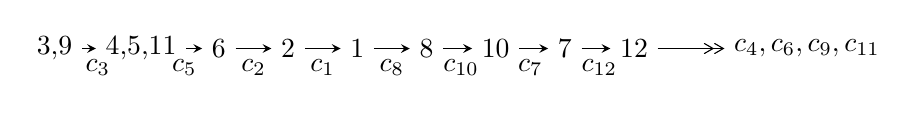
\begin{tikzpicture}[x=25pt, y=7pt]
	% node
	\node (A0) at (-1/8, 0) {3,9};
	\node (A1) at (9/8, 0) {4,5,11};
	\node (A2) at (9/4, 0) {6};
	\node (A3) at (13/4, 0) {2};
	\node (A4) at (17/4, 0) {1};
	\node (A5) at (21/4, 0) {8};
	\node (A6) at (25/4, 0) {10};
	\node (A7) at (29/4, 0) {7};
	\node (A8) at (33/4, 0) {12};
	\node (C1) at (1/2, -1) {$c_{3}$};
	\node (C2) at (7/4, -1) {$c_{5}$};
	\node (C3) at (11/4, -1) {$c_{2}$};
	\node (C4) at (15/4, -1) {$c_{1}$};
	\node (C5) at (19/4, -1) {$c_{8}$};
	\node (C6) at (23/4, -1) {$c_{10}$};
	\node (C7) at (27/4, -1) {$c_{7}$};
	\node (C8) at (31/4, -1) {$c_{12}$};
	\node (A9) at (43/4, 0) {$c_{4},c_{6},c_{9},c_{11}$};

	% edge
	\draw[->,>=stealth]	
	(A0) edge (A1) (A1) edge (A2) (A2) edge (A3) (A3) edge (A4) (A4) edge (A5) (A5) edge (A6) (A6) edge (A7) (A7) edge (A8) ;
	\draw[->>,>={angle 60}]	
	(A8) edge (A9);
\end{tikzpicture} \\ 

\end{tabular} \\

\footnotetext{
The image of knot diagram is generated by the software ``\textbf{Draw programme}" developed by Andrew Bartholomew(\url{http://www.layer8.co.uk/maths/draw/index.htm\#Running-draw}), where we modified some parts for our purpose(\url{https://github.com/CATsTAILs/LinksPainter}).
}\phantom \\ \newline 
\centering \textbf{Ideals for irreducible components\footnotemark of $X_{\text{par}}$} 
 
\begin{align*}
I^u_{1}&=\langle 
-4.12031\times10^{34} u^{30}-2.31311\times10^{35} u^{29}+\cdots+1.08242\times10^{37} d-4.05250\times10^{35},\\
\phantom{I^u_{1}}&\phantom{= \langle  }-3.25140\times10^{35} u^{30}-1.04293\times10^{36} u^{29}+\cdots+2.16483\times10^{37} c-2.49953\times10^{37},\\
\phantom{I^u_{1}}&\phantom{= \langle  }-6.96435\times10^{33} u^{30}+1.25405\times10^{34} u^{29}+\cdots+1.08242\times10^{37} b-4.63583\times10^{36},\\
\phantom{I^u_{1}}&\phantom{= \langle  }9.28423\times10^{34} u^{30}+2.43126\times10^{35} u^{29}+\cdots+2.16483\times10^{37} a-1.72516\times10^{37},\;u^{31}+3 u^{30}+\cdots+64 u+32\rangle \\
I^u_{2}&=\langle 
114533971308 u^{22} a-295693377683 u^{22}+\cdots+309089289992 a-1727678279402,\\
\phantom{I^u_{2}}&\phantom{= \langle  }-106328835549 u^{22} a-37415285413 u^{22}+\cdots-881316945982 a-268636021714,\\
\phantom{I^u_{2}}&\phantom{= \langle  }-38636161249 u^{22} a+6684998365 u^{22}+\cdots+212657671098 a-31359529106,\\
\phantom{I^u_{2}}&\phantom{= \langle  }709294494705 u^{22} a-467986206381 u^{22}+\cdots+1120177291630 a+112735730394,\\
\phantom{I^u_{2}}&\phantom{= \langle  }u^{23}- u^{22}+\cdots+8 u+4\rangle \\
\\
I^v_{1}&=\langle 
a,\;d,\;c- v,\;b-1,\;v^2- v+1\rangle \\
I^v_{2}&=\langle 
c,\;d+v-1,\;b,\;a-1,\;v^2- v+1\rangle \\
I^v_{3}&=\langle 
a,\;d+1,\;c+a,\;b-1,\;v+1\rangle \\
I^v_{4}&=\langle 
a,\;a^2 d+c^2 v-2 c a- c v+a+v,\;d v-1,\;c^2 v^2-2 c a v- v^2 c+a^2+a v+v^2,\;b-1\rangle \\
\end{align*}
\raggedright * 5 irreducible components of $\dim_{\mathbb{C}}=0$, with total 82 representations.\\
\raggedright * 1 irreducible components of $\dim_{\mathbb{C}}=1$ \\
\footnotetext{All coefficients of polynomials are rational numbers. But the coefficients are sometimes approximated in decimal forms when there is not enough margin.}
\newpage
\renewcommand{\arraystretch}{1}
\centering \section*{I. $I^u_{1}= \langle -4.12\times10^{34} u^{30}-2.31\times10^{35} u^{29}+\cdots+1.08\times10^{37} d-4.05\times10^{35},\;-3.25\times10^{35} u^{30}-1.04\times10^{36} u^{29}+\cdots+2.16\times10^{37} c-2.50\times10^{37},\;-6.96\times10^{33} u^{30}+1.25\times10^{34} u^{29}+\cdots+1.08\times10^{37} b-4.64\times10^{36},\;9.28\times10^{34} u^{30}+2.43\times10^{35} u^{29}+\cdots+2.16\times10^{37} a-1.73\times10^{37},\;u^{31}+3 u^{30}+\cdots+64 u+32 \rangle$}
\flushleft \textbf{(i) Arc colorings}\\
\begin{tabular}{m{7pt} m{180pt} m{7pt} m{180pt} }
\flushright $a_{3}=$&$\begin{pmatrix}1\\0\end{pmatrix}$ \\
\flushright $a_{9}=$&$\begin{pmatrix}0\\u\end{pmatrix}$ \\
\flushright $a_{4}=$&$\begin{pmatrix}1\\u^2\end{pmatrix}$ \\
\flushright $a_{5}=$&$\begin{pmatrix}-0.00428866 u^{30}-0.0112307 u^{29}+\cdots-0.0728208 u+0.796905\\0.000643408 u^{30}-0.00115856 u^{29}+\cdots-0.160798 u+0.428286\end{pmatrix}$ \\
\flushright $a_{11}=$&$\begin{pmatrix}0.0150192 u^{30}+0.0481763 u^{29}+\cdots+0.421287 u+1.15461\\0.00380659 u^{30}+0.0213699 u^{29}+\cdots+0.391169 u+0.0374394\end{pmatrix}$ \\
\flushright $a_{6}=$&$\begin{pmatrix}0.0281261 u^{30}+0.0745920 u^{29}+\cdots-0.311221 u+1.89333\\-0.000510466 u^{30}-0.00677158 u^{29}+\cdots-0.959619 u+0.547953\end{pmatrix}$ \\
\flushright $a_{2}=$&$\begin{pmatrix}-0.00428866 u^{30}-0.0112307 u^{29}+\cdots-0.0728208 u+0.796905\\0.00311868 u^{30}+0.0115274 u^{29}+\cdots+0.193379 u-0.480614\end{pmatrix}$ \\
\flushright $a_{1}=$&$\begin{pmatrix}-0.00116998 u^{30}+0.000296647 u^{29}+\cdots+0.120558 u+0.316290\\0.00311868 u^{30}+0.0115274 u^{29}+\cdots+0.193379 u-0.480614\end{pmatrix}$ \\
\flushright $a_{8}=$&$\begin{pmatrix}u\\u\end{pmatrix}$ \\
\flushright $a_{10}=$&$\begin{pmatrix}0.0150192 u^{30}+0.0481763 u^{29}+\cdots+0.421287 u+1.15461\\0.00163526 u^{30}+0.00866787 u^{29}+\cdots+1.07138 u+0.137237\end{pmatrix}$ \\
\flushright $a_{7}=$&$\begin{pmatrix}-0.0133839 u^{30}-0.0395084 u^{29}+\cdots+0.650092 u-1.01737\\0.00163526 u^{30}+0.00866787 u^{29}+\cdots+1.07138 u+0.137237\end{pmatrix}$ \\
\flushright $a_{12}=$&$\begin{pmatrix}0.0125773 u^{30}+0.0545128 u^{29}+\cdots+1.19403 u+1.13915\\-0.00454622 u^{30}+0.00263169 u^{29}+\cdots-0.487370 u-0.916371\end{pmatrix}$\\&\end{tabular}
\flushleft \textbf{(ii) Obstruction class $= -1$}\\~\\
\flushleft \textbf{(iii) Cusp Shapes $= -0.0330834 u^{30}-0.0743041 u^{29}+\cdots-9.35750 u-13.8824$}\\~\\
\newpage\renewcommand{\arraystretch}{1}
\flushleft \textbf{(iv) u-Polynomials at the component}\newline \\
\begin{tabular}{m{50pt}|m{274pt}}
Crossings & \hspace{64pt}u-Polynomials at each crossing \\
\hline $$\begin{aligned}c_{1},c_{10}\end{aligned}$$&$\begin{aligned}
&u^{31}+11 u^{30}+\cdots+21 u+1
\end{aligned}$\\
\hline $$\begin{aligned}c_{2},c_{4},c_{7}\\c_{9}\end{aligned}$$&$\begin{aligned}
&u^{31}-5 u^{30}+\cdots-3 u+1
\end{aligned}$\\
\hline $$\begin{aligned}c_{3},c_{8}\end{aligned}$$&$\begin{aligned}
&u^{31}+3 u^{30}+\cdots+64 u+32
\end{aligned}$\\
\hline $$\begin{aligned}c_{5}\end{aligned}$$&$\begin{aligned}
&u^{31}+u^{30}+\cdots+128 u+548
\end{aligned}$\\
\hline $$\begin{aligned}c_{6},c_{12}\end{aligned}$$&$\begin{aligned}
&u^{31}- u^{30}+\cdots+8 u+4
\end{aligned}$\\
\hline $$\begin{aligned}c_{11}\end{aligned}$$&$\begin{aligned}
&u^{31}-15 u^{30}+\cdots+120 u+16
\end{aligned}$\\
\hline
\end{tabular}\\~\\
\newpage\renewcommand{\arraystretch}{1}
\flushleft \textbf{(v) Riley Polynomials at the component}\newline \\
\begin{tabular}{m{50pt}|m{274pt}}
Crossings & \hspace{64pt}Riley Polynomials at each crossing \\
\hline $$\begin{aligned}c_{1},c_{10}\end{aligned}$$&$\begin{aligned}
&y^{31}+29 y^{30}+\cdots+61 y-1
\end{aligned}$\\
\hline $$\begin{aligned}c_{2},c_{4},c_{7}\\c_{9}\end{aligned}$$&$\begin{aligned}
&y^{31}-11 y^{30}+\cdots+21 y-1
\end{aligned}$\\
\hline $$\begin{aligned}c_{3},c_{8}\end{aligned}$$&$\begin{aligned}
&y^{31}+15 y^{30}+\cdots+1024 y-1024
\end{aligned}$\\
\hline $$\begin{aligned}c_{5}\end{aligned}$$&$\begin{aligned}
&y^{31}-9 y^{30}+\cdots+4451896 y-300304
\end{aligned}$\\
\hline $$\begin{aligned}c_{6},c_{12}\end{aligned}$$&$\begin{aligned}
&y^{31}+15 y^{30}+\cdots+120 y-16
\end{aligned}$\\
\hline $$\begin{aligned}c_{11}\end{aligned}$$&$\begin{aligned}
&y^{31}+3 y^{30}+\cdots+25888 y-256
\end{aligned}$\\
\hline
\end{tabular}\\~\\
\newpage\flushleft \textbf{(vi) Complex Volumes and Cusp Shapes}
$$\begin{array}{c|c|c}  
\text{Solutions to }I^u_{1}& \I (\text{vol} + \sqrt{-1}CS) & \text{Cusp shape}\\
 \hline 
\begin{aligned}
u &= \phantom{-}0.753219 + 0.379837 I \\
a &= \phantom{-}0.685053 - 0.287784 I \\
b &= \phantom{-}0.240774 + 0.521238 I \\
c &= \phantom{-}0.092235 - 0.379751 I \\
d &= \phantom{-}0.881620 - 0.064438 I\end{aligned}
 & \phantom{-}1.42006 - 1.96537 I & -1.93692 + 5.44006 I \\ \hline\begin{aligned}
u &= \phantom{-}0.753219 - 0.379837 I \\
a &= \phantom{-}0.685053 + 0.287784 I \\
b &= \phantom{-}0.240774 - 0.521238 I \\
c &= \phantom{-}0.092235 + 0.379751 I \\
d &= \phantom{-}0.881620 + 0.064438 I\end{aligned}
 & \phantom{-}1.42006 + 1.96537 I & -1.93692 - 5.44006 I \\ \hline\begin{aligned}
u &= -0.337564 + 1.132290 I \\
a &= \phantom{-}0.17117 - 1.61585 I \\
b &= -0.935169 + 0.612003 I \\
c &= \phantom{-}1.049310 + 0.128753 I \\
d &= \phantom{-}0.644525 - 0.213262 I\end{aligned}
 & -0.45247 + 2.02679 I & -7.73031 - 3.42583 I \\ \hline\begin{aligned}
u &= -0.337564 - 1.132290 I \\
a &= \phantom{-}0.17117 + 1.61585 I \\
b &= -0.935169 - 0.612003 I \\
c &= \phantom{-}1.049310 - 0.128753 I \\
d &= \phantom{-}0.644525 + 0.213262 I\end{aligned}
 & -0.45247 - 2.02679 I & -7.73031 + 3.42583 I \\ \hline\begin{aligned}
u &= \phantom{-}1.121020 + 0.424146 I \\
a &= \phantom{-}0.460731 + 0.138106 I \\
b &= \phantom{-}0.991521 - 0.596969 I \\
c &= -0.139555 + 1.108810 I \\
d &= -0.74679 + 1.41149 I\end{aligned}
 & -1.55877 + 4.66712 I & -11.51750 - 4.56967 I \\ \hline\begin{aligned}
u &= \phantom{-}1.121020 - 0.424146 I \\
a &= \phantom{-}0.460731 - 0.138106 I \\
b &= \phantom{-}0.991521 + 0.596969 I \\
c &= -0.139555 - 1.108810 I \\
d &= -0.74679 - 1.41149 I\end{aligned}
 & -1.55877 - 4.66712 I & -11.51750 + 4.56967 I\\
 \hline 
 \end{array}$$\newpage$$\begin{array}{c|c|c}  
\text{Solutions to }I^u_{1}& \I (\text{vol} + \sqrt{-1}CS) & \text{Cusp shape}\\
 \hline 
\begin{aligned}
u &= \phantom{-}0.698083 + 0.364692 I \\
a &= \phantom{-}0.498679 + 0.078631 I \\
b &= \phantom{-}0.956651 - 0.308522 I \\
c &= -0.575750 + 1.146380 I \\
d &= -0.468258 + 0.349784 I\end{aligned}
 & -3.68376 + 3.19069 I & -14.6846 - 5.1485 I \\ \hline\begin{aligned}
u &= \phantom{-}0.698083 - 0.364692 I \\
a &= \phantom{-}0.498679 - 0.078631 I \\
b &= \phantom{-}0.956651 + 0.308522 I \\
c &= -0.575750 - 1.146380 I \\
d &= -0.468258 - 0.349784 I\end{aligned}
 & -3.68376 - 3.19069 I & -14.6846 + 5.1485 I \\ \hline\begin{aligned}
u &= -1.235540 + 0.189024 I \\
a &= \phantom{-}0.472913 - 0.179552 I \\
b &= \phantom{-}0.848142 + 0.701686 I \\
c &= \phantom{-}0.035497 + 0.968785 I \\
d &= -0.04493 + 1.73894 I\end{aligned}
 & \phantom{-}2.56816 - 1.34649 I & -5.38369 + 2.07194 I \\ \hline\begin{aligned}
u &= -1.235540 - 0.189024 I \\
a &= \phantom{-}0.472913 + 0.179552 I \\
b &= \phantom{-}0.848142 - 0.701686 I \\
c &= \phantom{-}0.035497 - 0.968785 I \\
d &= -0.04493 - 1.73894 I\end{aligned}
 & \phantom{-}2.56816 + 1.34649 I & -5.38369 - 2.07194 I \\ \hline\begin{aligned}
u &= \phantom{-}0.464557 + 1.163760 I \\
a &= -0.05406 + 1.60814 I \\
b &= -1.020880 - 0.621136 I \\
c &= -1.134180 + 0.111276 I \\
d &= -0.725633 - 0.668879 I\end{aligned}
 & -1.15318 - 7.72517 I & -9.61403 + 8.29170 I \\ \hline\begin{aligned}
u &= \phantom{-}0.464557 - 1.163760 I \\
a &= -0.05406 - 1.60814 I \\
b &= -1.020880 + 0.621136 I \\
c &= -1.134180 - 0.111276 I \\
d &= -0.725633 + 0.668879 I\end{aligned}
 & -1.15318 + 7.72517 I & -9.61403 - 8.29170 I\\
 \hline 
 \end{array}$$\newpage$$\begin{array}{c|c|c}  
\text{Solutions to }I^u_{1}& \I (\text{vol} + \sqrt{-1}CS) & \text{Cusp shape}\\
 \hline 
\begin{aligned}
u &= -1.253240 + 0.506936 I \\
a &= \phantom{-}0.439439 - 0.143874 I \\
b &= \phantom{-}1.055310 + 0.672917 I \\
c &= \phantom{-}0.059221 + 1.157240 I \\
d &= \phantom{-}1.07042 + 1.84800 I\end{aligned}
 & \phantom{-}1.12377 - 9.51847 I & -8.01541 + 7.69926 I \\ \hline\begin{aligned}
u &= -1.253240 - 0.506936 I \\
a &= \phantom{-}0.439439 + 0.143874 I \\
b &= \phantom{-}1.055310 - 0.672917 I \\
c &= \phantom{-}0.059221 - 1.157240 I \\
d &= \phantom{-}1.07042 - 1.84800 I\end{aligned}
 & \phantom{-}1.12377 + 9.51847 I & -8.01541 - 7.69926 I \\ \hline\begin{aligned}
u &= \phantom{-}0.223678 + 1.371700 I \\
a &= \phantom{-}0.413752 - 0.939419 I \\
b &= -0.607334 + 0.891545 I \\
c &= \phantom{-}0.818360 - 0.177114 I \\
d &= -0.009021 + 1.183990 I\end{aligned}
 & \phantom{-}4.93468 + 0.57606 I & -5.79676 - 1.97891 I \\ \hline\begin{aligned}
u &= \phantom{-}0.223678 - 1.371700 I \\
a &= \phantom{-}0.413752 + 0.939419 I \\
b &= -0.607334 - 0.891545 I \\
c &= \phantom{-}0.818360 + 0.177114 I \\
d &= -0.009021 - 1.183990 I\end{aligned}
 & \phantom{-}4.93468 - 0.57606 I & -5.79676 + 1.97891 I \\ \hline\begin{aligned}
u &= -0.591801\phantom{ +0.000000I} \\
a &= \phantom{-}0.699591\phantom{ +0.000000I} \\
b &= \phantom{-}0.429406\phantom{ +0.000000I} \\
c &= \phantom{-}0.311574\phantom{ +0.000000I} \\
d &= -0.304897\phantom{ +0.000000I}\end{aligned}
 & -0.834149\phantom{ +0.000000I} & -11.9720\phantom{ +0.000000I} \\ \hline\begin{aligned}
u &= -0.540907 + 0.236782 I \\
a &= \phantom{-}0.518602 - 0.047373 I \\
b &= \phantom{-}0.912302 + 0.174686 I \\
c &= \phantom{-}1.02746 + 1.03902 I \\
d &= \phantom{-}0.239860 + 0.130978 I\end{aligned}
 & -3.12062 + 1.49349 I & -14.4230 - 1.8126 I\\
 \hline 
 \end{array}$$\newpage$$\begin{array}{c|c|c}  
\text{Solutions to }I^u_{1}& \I (\text{vol} + \sqrt{-1}CS) & \text{Cusp shape}\\
 \hline 
\begin{aligned}
u &= -0.540907 - 0.236782 I \\
a &= \phantom{-}0.518602 + 0.047373 I \\
b &= \phantom{-}0.912302 - 0.174686 I \\
c &= \phantom{-}1.02746 - 1.03902 I \\
d &= \phantom{-}0.239860 - 0.130978 I\end{aligned}
 & -3.12062 - 1.49349 I & -14.4230 + 1.8126 I \\ \hline\begin{aligned}
u &= \phantom{-}0.067118 + 0.557682 I \\
a &= \phantom{-}1.45537 - 0.23813 I \\
b &= -0.330807 + 0.109496 I \\
c &= \phantom{-}0.107319 + 0.187646 I \\
d &= \phantom{-}0.183545 + 0.746172 I\end{aligned}
 & -0.46111 + 2.29513 I & -1.47827 - 3.85950 I \\ \hline\begin{aligned}
u &= \phantom{-}0.067118 - 0.557682 I \\
a &= \phantom{-}1.45537 + 0.23813 I \\
b &= -0.330807 - 0.109496 I \\
c &= \phantom{-}0.107319 - 0.187646 I \\
d &= \phantom{-}0.183545 - 0.746172 I\end{aligned}
 & -0.46111 - 2.29513 I & -1.47827 + 3.85950 I \\ \hline\begin{aligned}
u &= \phantom{-}0.71578 + 1.28059 I \\
a &= -0.37486 + 1.39000 I \\
b &= -1.180860 - 0.670647 I \\
c &= -1.256580 + 0.035321 I \\
d &= -0.69622 - 1.82856 I\end{aligned}
 & \phantom{-}1.16605 - 11.32090 I & -10.43454 + 6.71502 I \\ \hline\begin{aligned}
u &= \phantom{-}0.71578 - 1.28059 I \\
a &= -0.37486 - 1.39000 I \\
b &= -1.180860 + 0.670647 I \\
c &= -1.256580 - 0.035321 I \\
d &= -0.69622 + 1.82856 I\end{aligned}
 & \phantom{-}1.16605 + 11.32090 I & -10.43454 - 6.71502 I \\ \hline\begin{aligned}
u &= -0.39077 + 1.46203 I \\
a &= \phantom{-}0.382686 + 0.821951 I \\
b &= -0.534475 - 0.999877 I \\
c &= -0.804151 - 0.273493 I \\
d &= -0.06766 + 1.69998 I\end{aligned}
 & \phantom{-}8.24554 + 4.31764 I & -2.71892 - 1.88458 I\\
 \hline 
 \end{array}$$\newpage$$\begin{array}{c|c|c}  
\text{Solutions to }I^u_{1}& \I (\text{vol} + \sqrt{-1}CS) & \text{Cusp shape}\\
 \hline 
\begin{aligned}
u &= -0.39077 - 1.46203 I \\
a &= \phantom{-}0.382686 - 0.821951 I \\
b &= -0.534475 + 0.999877 I \\
c &= -0.804151 + 0.273493 I \\
d &= -0.06766 - 1.69998 I\end{aligned}
 & \phantom{-}8.24554 - 4.31764 I & -2.71892 + 1.88458 I \\ \hline\begin{aligned}
u &= -0.79393 + 1.30401 I \\
a &= -0.444220 - 1.327190 I \\
b &= -1.226790 + 0.677567 I \\
c &= \phantom{-}1.286380 + 0.018874 I \\
d &= \phantom{-}0.74586 - 2.20933 I\end{aligned}
 & \phantom{-}3.7041 + 16.8176 I & -8.02968 - 10.05725 I \\ \hline\begin{aligned}
u &= -0.79393 - 1.30401 I \\
a &= -0.444220 + 1.327190 I \\
b &= -1.226790 - 0.677567 I \\
c &= \phantom{-}1.286380 - 0.018874 I \\
d &= \phantom{-}0.74586 + 2.20933 I\end{aligned}
 & \phantom{-}3.7041 - 16.8176 I & -8.02968 + 10.05725 I \\ \hline\begin{aligned}
u &= -0.62073 + 1.40356 I \\
a &= -0.237422 - 1.289560 I \\
b &= -1.138090 + 0.750034 I \\
c &= \phantom{-}1.210460 - 0.013304 I \\
d &= \phantom{-}0.01599 - 1.62087 I\end{aligned}
 & \phantom{-}6.51517 + 8.00123 I & -4.81025 - 4.92455 I \\ \hline\begin{aligned}
u &= -0.62073 - 1.40356 I \\
a &= -0.237422 + 1.289560 I \\
b &= -1.138090 - 0.750034 I \\
c &= \phantom{-}1.210460 + 0.013304 I \\
d &= \phantom{-}0.01599 + 1.62087 I\end{aligned}
 & \phantom{-}6.51517 - 8.00123 I & -4.81025 + 4.92455 I \\ \hline\begin{aligned}
u &= -0.07489 + 1.53753 I \\
a &= \phantom{-}0.262372 + 0.979829 I \\
b &= -0.744999 - 0.952303 I \\
c &= -0.931800 - 0.183463 I \\
d &= \phantom{-}0.629132 + 0.977280 I\end{aligned}
 & \phantom{-}9.13328 - 4.81435 I & -2.44035 + 4.85668 I\\
 \hline 
 \end{array}$$\newpage$$\begin{array}{c|c|c}  
\text{Solutions to }I^u_{1}& \I (\text{vol} + \sqrt{-1}CS) & \text{Cusp shape}\\
 \hline 
\begin{aligned}
u &= -0.07489 - 1.53753 I \\
a &= \phantom{-}0.262372 - 0.979829 I \\
b &= -0.744999 + 0.952303 I \\
c &= -0.931800 + 0.183463 I \\
d &= \phantom{-}0.629132 - 0.977280 I\end{aligned}
 & \phantom{-}9.13328 + 4.81435 I & -2.44035 - 4.85668 I\\
 \hline 
 \end{array}$$\newpage\newpage\renewcommand{\arraystretch}{1}
\centering \section*{II. $I^u_{2}= \langle 1.15\times10^{11} a u^{22}-2.96\times10^{11} u^{22}+\cdots+3.09\times10^{11} a-1.73\times10^{12},\;-1.06\times10^{11} a u^{22}-3.74\times10^{10} u^{22}+\cdots-8.81\times10^{11} a-2.69\times10^{11},\;-3.86\times10^{10} a u^{22}+6.68\times10^{9} u^{22}+\cdots+2.13\times10^{11} a-3.14\times10^{10},\;7.09\times10^{11} a u^{22}-4.68\times10^{11} u^{22}+\cdots+1.12\times10^{12} a+1.13\times10^{11},\;u^{23}- u^{22}+\cdots+8 u+4 \rangle$}
\flushleft \textbf{(i) Arc colorings}\\
\begin{tabular}{m{7pt} m{180pt} m{7pt} m{180pt} }
\flushright $a_{3}=$&$\begin{pmatrix}1\\0\end{pmatrix}$ \\
\flushright $a_{9}=$&$\begin{pmatrix}0\\u\end{pmatrix}$ \\
\flushright $a_{4}=$&$\begin{pmatrix}1\\u^2\end{pmatrix}$ \\
\flushright $a_{5}=$&$\begin{pmatrix}a\\0.134392 a u^{22}-0.0232531 u^{22}+\cdots-0.739709 a+0.109081\end{pmatrix}$ \\
\flushright $a_{11}=$&$\begin{pmatrix}0.184927 a u^{22}+0.0650727 u^{22}+\cdots+1.53279 a+0.467212\\-0.199198 a u^{22}+0.514270 u^{22}+\cdots-0.537569 a+3.00478\end{pmatrix}$ \\
\flushright $a_{6}=$&$\begin{pmatrix}0.0536818 a u^{22}-0.109233 u^{22}+\cdots+1.15888 a-1.35137\\0.147105 a u^{22}-0.215441 u^{22}+\cdots-2.41722 a-0.588197\end{pmatrix}$ \\
\flushright $a_{2}=$&$\begin{pmatrix}a\\-0.134392 a u^{22}+0.0232531 u^{22}+\cdots+0.739709 a-0.109081\end{pmatrix}$ \\
\flushright $a_{1}=$&$\begin{pmatrix}-0.134392 a u^{22}+0.0232531 u^{22}+\cdots+1.73971 a-0.109081\\-0.134392 a u^{22}+0.0232531 u^{22}+\cdots+0.739709 a-0.109081\end{pmatrix}$ \\
\flushright $a_{8}=$&$\begin{pmatrix}u\\u\end{pmatrix}$ \\
\flushright $a_{10}=$&$\begin{pmatrix}0.184927 a u^{22}+0.0650727 u^{22}+\cdots+1.53279 a+0.467212\\0.315073 u^{22}-0.449465 u^{21}+\cdots+3.96032 u+2.46721\end{pmatrix}$ \\
\flushright $a_{7}=$&$\begin{pmatrix}-0.184927 a u^{22}+0.250000 u^{22}+\cdots-1.53279 a+2\\0.315073 u^{22}-0.449465 u^{21}+\cdots+3.96032 u+2.46721\end{pmatrix}$ \\
\flushright $a_{12}=$&$\begin{pmatrix}-0.0514525 a u^{22}+0.220414 u^{22}+\cdots+1.82586 a+0.884563\\-0.655758 a u^{22}+0.669612 u^{22}+\cdots-0.373694 a+3.42213\end{pmatrix}$\\&\end{tabular}
\flushleft \textbf{(ii) Obstruction class $= -1$}\\~\\
\flushleft \textbf{(iii) Cusp Shapes $= -\frac{173371509589}{143744120962} u^{22}+\frac{241902270957}{143744120962} u^{21}+\cdots+\frac{379864412243}{143744120962} u-\frac{545150434432}{71872060481}$}\\~\\
\newpage\renewcommand{\arraystretch}{1}
\flushleft \textbf{(iv) u-Polynomials at the component}\newline \\
\begin{tabular}{m{50pt}|m{274pt}}
Crossings & \hspace{64pt}u-Polynomials at each crossing \\
\hline $$\begin{aligned}c_{1},c_{10}\end{aligned}$$&$\begin{aligned}
&u^{46}+23 u^{45}+\cdots+288 u+256
\end{aligned}$\\
\hline $$\begin{aligned}c_{2},c_{4},c_{7}\\c_{9}\end{aligned}$$&$\begin{aligned}
&u^{46}-3 u^{45}+\cdots-56 u+16
\end{aligned}$\\
\hline $$\begin{aligned}c_{3},c_{8}\end{aligned}$$&$\begin{aligned}
&(u^{23}- u^{22}+\cdots+8 u+4)^{2}
\end{aligned}$\\
\hline $$\begin{aligned}c_{5}\end{aligned}$$&$\begin{aligned}
&(u^{23}+2 u^{22}+\cdots+18 u+9)^{2}
\end{aligned}$\\
\hline $$\begin{aligned}c_{6},c_{12}\end{aligned}$$&$\begin{aligned}
&(u^{23}-2 u^{22}+\cdots-2 u+1)^{2}
\end{aligned}$\\
\hline $$\begin{aligned}c_{11}\end{aligned}$$&$\begin{aligned}
&(u^{23}-12 u^{22}+\cdots-2 u+1)^{2}
\end{aligned}$\\
\hline
\end{tabular}\\~\\
\newpage\renewcommand{\arraystretch}{1}
\flushleft \textbf{(v) Riley Polynomials at the component}\newline \\
\begin{tabular}{m{50pt}|m{274pt}}
Crossings & \hspace{64pt}Riley Polynomials at each crossing \\
\hline $$\begin{aligned}c_{1},c_{10}\end{aligned}$$&$\begin{aligned}
&y^{46}-3 y^{45}+\cdots-2449920 y+65536
\end{aligned}$\\
\hline $$\begin{aligned}c_{2},c_{4},c_{7}\\c_{9}\end{aligned}$$&$\begin{aligned}
&y^{46}-23 y^{45}+\cdots-288 y+256
\end{aligned}$\\
\hline $$\begin{aligned}c_{3},c_{8}\end{aligned}$$&$\begin{aligned}
&(y^{23}+15 y^{22}+\cdots-40 y-16)^{2}
\end{aligned}$\\
\hline $$\begin{aligned}c_{5}\end{aligned}$$&$\begin{aligned}
&(y^{23}-12 y^{22}+\cdots-450 y-81)^{2}
\end{aligned}$\\
\hline $$\begin{aligned}c_{6},c_{12}\end{aligned}$$&$\begin{aligned}
&(y^{23}+12 y^{22}+\cdots-2 y-1)^{2}
\end{aligned}$\\
\hline $$\begin{aligned}c_{11}\end{aligned}$$&$\begin{aligned}
&(y^{23}+24 y^{21}+\cdots+10 y-1)^{2}
\end{aligned}$\\
\hline
\end{tabular}\\~\\
\newpage\flushleft \textbf{(vi) Complex Volumes and Cusp Shapes}
$$\begin{array}{c|c|c}  
\text{Solutions to }I^u_{2}& \I (\text{vol} + \sqrt{-1}CS) & \text{Cusp shape}\\
 \hline 
\begin{aligned}
u &= -0.969482\phantom{ +0.000000I} \\
a &= \phantom{-}0.546696 + 0.177229 I \\
b &= \phantom{-}0.655217 - 0.536590 I \\
c &= \phantom{-}0.145831 + 0.725301 I \\
d &= -0.392946 + 0.853527 I\end{aligned}
 & -0.502753\phantom{ +0.000000I} & -9.67610\phantom{ +0.000000I} \\ \hline\begin{aligned}
u &= -0.969482\phantom{ +0.000000I} \\
a &= \phantom{-}0.546696 - 0.177229 I \\
b &= \phantom{-}0.655217 + 0.536590 I \\
c &= \phantom{-}0.145831 - 0.725301 I \\
d &= -0.392946 - 0.853527 I\end{aligned}
 & -0.502753\phantom{ +0.000000I} & -9.67610\phantom{ +0.000000I} \\ \hline\begin{aligned}
u &= \phantom{-}0.308169 + 0.985429 I \\
a &= \phantom{-}0.430219 + 0.027076 I \\
b &= \phantom{-}1.315230 - 0.145711 I \\
c &= -1.015110 + 0.244961 I \\
d &= -1.008850 + 0.100976 I\end{aligned}
 & -2.62555 - 2.00215 I & -10.76412 + 3.62705 I \\ \hline\begin{aligned}
u &= \phantom{-}0.308169 + 0.985429 I \\
a &= \phantom{-}0.35592 + 1.88659 I \\
b &= -0.903437 - 0.511840 I \\
c &= -0.13961 + 1.69019 I \\
d &= -0.798336 - 1.133280 I\end{aligned}
 & -2.62555 - 2.00215 I & -10.76412 + 3.62705 I \\ \hline\begin{aligned}
u &= \phantom{-}0.308169 - 0.985429 I \\
a &= \phantom{-}0.430219 - 0.027076 I \\
b &= \phantom{-}1.315230 + 0.145711 I \\
c &= -1.015110 - 0.244961 I \\
d &= -1.008850 - 0.100976 I\end{aligned}
 & -2.62555 + 2.00215 I & -10.76412 - 3.62705 I \\ \hline\begin{aligned}
u &= \phantom{-}0.308169 - 0.985429 I \\
a &= \phantom{-}0.35592 - 1.88659 I \\
b &= -0.903437 + 0.511840 I \\
c &= -0.13961 - 1.69019 I \\
d &= -0.798336 + 1.133280 I\end{aligned}
 & -2.62555 + 2.00215 I & -10.76412 - 3.62705 I\\
 \hline 
 \end{array}$$\newpage$$\begin{array}{c|c|c}  
\text{Solutions to }I^u_{2}& \I (\text{vol} + \sqrt{-1}CS) & \text{Cusp shape}\\
 \hline 
\begin{aligned}
u &= -0.107498 + 1.054050 I \\
a &= \phantom{-}0.716893 + 1.112390 I \\
b &= -0.590662 - 0.635162 I \\
c &= \phantom{-}0.855712 + 0.135596 I \\
d &= \phantom{-}0.567042 + 0.449517 I\end{aligned}
 & \phantom{-}0.12065 + 2.74438 I & -5.99863 - 3.42075 I \\ \hline\begin{aligned}
u &= -0.107498 + 1.054050 I \\
a &= \phantom{-}0.60269 - 1.46286 I \\
b &= -0.759232 + 0.584397 I \\
c &= -0.709753 + 0.020633 I \\
d &= -0.464556 + 0.774218 I\end{aligned}
 & \phantom{-}0.12065 + 2.74438 I & -5.99863 - 3.42075 I \\ \hline\begin{aligned}
u &= -0.107498 - 1.054050 I \\
a &= \phantom{-}0.716893 - 1.112390 I \\
b &= -0.590662 + 0.635162 I \\
c &= \phantom{-}0.855712 - 0.135596 I \\
d &= \phantom{-}0.567042 - 0.449517 I\end{aligned}
 & \phantom{-}0.12065 - 2.74438 I & -5.99863 + 3.42075 I \\ \hline\begin{aligned}
u &= -0.107498 - 1.054050 I \\
a &= \phantom{-}0.60269 + 1.46286 I \\
b &= -0.759232 - 0.584397 I \\
c &= -0.709753 - 0.020633 I \\
d &= -0.464556 - 0.774218 I\end{aligned}
 & \phantom{-}0.12065 - 2.74438 I & -5.99863 + 3.42075 I \\ \hline\begin{aligned}
u &= -0.000983 + 1.149400 I \\
a &= \phantom{-}0.547631 - 1.231120 I \\
b &= -0.698366 + 0.678096 I \\
c &= \phantom{-}0.00032 + 1.69379 I \\
d &= \phantom{-}0.00309 - 1.75784 I\end{aligned}
 & \phantom{-}0.86138 - 1.33135 I & -4.84050 + 0.67575 I \\ \hline\begin{aligned}
u &= -0.000983 + 1.149400 I \\
a &= \phantom{-}0.417486 - 0.000081 I \\
b &= \phantom{-}1.395290 + 0.000467 I \\
c &= \phantom{-}0.824032 + 0.023570 I \\
d &= \phantom{-}0.325917 + 0.597656 I\end{aligned}
 & \phantom{-}0.86138 - 1.33135 I & -4.84050 + 0.67575 I\\
 \hline 
 \end{array}$$\newpage$$\begin{array}{c|c|c}  
\text{Solutions to }I^u_{2}& \I (\text{vol} + \sqrt{-1}CS) & \text{Cusp shape}\\
 \hline 
\begin{aligned}
u &= -0.000983 - 1.149400 I \\
a &= \phantom{-}0.547631 + 1.231120 I \\
b &= -0.698366 - 0.678096 I \\
c &= \phantom{-}0.00032 - 1.69379 I \\
d &= \phantom{-}0.00309 + 1.75784 I\end{aligned}
 & \phantom{-}0.86138 + 1.33135 I & -4.84050 - 0.67575 I \\ \hline\begin{aligned}
u &= -0.000983 - 1.149400 I \\
a &= \phantom{-}0.417486 + 0.000081 I \\
b &= \phantom{-}1.395290 - 0.000467 I \\
c &= \phantom{-}0.824032 - 0.023570 I \\
d &= \phantom{-}0.325917 - 0.597656 I\end{aligned}
 & \phantom{-}0.86138 + 1.33135 I & -4.84050 - 0.67575 I \\ \hline\begin{aligned}
u &= \phantom{-}1.222080 + 0.199525 I \\
a &= \phantom{-}0.508002 - 0.253270 I \\
b &= \phantom{-}0.576609 + 0.786036 I \\
c &= -0.046249 + 0.972025 I \\
d &= \phantom{-}0.00251 + 1.70085 I\end{aligned}
 & \phantom{-}2.55344 + 3.99588 I & -5.39099 - 3.49800 I \\ \hline\begin{aligned}
u &= \phantom{-}1.222080 + 0.199525 I \\
a &= \phantom{-}0.473795 + 0.176635 I \\
b &= \phantom{-}0.853067 - 0.690841 I \\
c &= \phantom{-}0.109495 - 0.759619 I \\
d &= \phantom{-}1.20097 - 1.25900 I\end{aligned}
 & \phantom{-}2.55344 + 3.99588 I & -5.39099 - 3.49800 I \\ \hline\begin{aligned}
u &= \phantom{-}1.222080 - 0.199525 I \\
a &= \phantom{-}0.508002 + 0.253270 I \\
b &= \phantom{-}0.576609 - 0.786036 I \\
c &= -0.046249 - 0.972025 I \\
d &= \phantom{-}0.00251 - 1.70085 I\end{aligned}
 & \phantom{-}2.55344 - 3.99588 I & -5.39099 + 3.49800 I \\ \hline\begin{aligned}
u &= \phantom{-}1.222080 - 0.199525 I \\
a &= \phantom{-}0.473795 - 0.176635 I \\
b &= \phantom{-}0.853067 + 0.690841 I \\
c &= \phantom{-}0.109495 + 0.759619 I \\
d &= \phantom{-}1.20097 + 1.25900 I\end{aligned}
 & \phantom{-}2.55344 - 3.99588 I & -5.39099 + 3.49800 I\\
 \hline 
 \end{array}$$\newpage$$\begin{array}{c|c|c}  
\text{Solutions to }I^u_{2}& \I (\text{vol} + \sqrt{-1}CS) & \text{Cusp shape}\\
 \hline 
\begin{aligned}
u &= -0.383777 + 1.192290 I \\
a &= \phantom{-}0.06728 - 1.54278 I \\
b &= -0.971785 + 0.646950 I \\
c &= \phantom{-}0.08568 + 1.62327 I \\
d &= \phantom{-}1.25576 - 1.64401 I\end{aligned}
 & \phantom{-}0.03073 + 6.47771 I & -7.22220 - 6.52194 I \\ \hline\begin{aligned}
u &= -0.383777 + 1.192290 I \\
a &= \phantom{-}0.411691 - 0.031373 I \\
b &= \phantom{-}1.41498 + 0.18404 I \\
c &= \phantom{-}1.084230 + 0.092026 I \\
d &= \phantom{-}0.516239 - 0.437185 I\end{aligned}
 & \phantom{-}0.03073 + 6.47771 I & -7.22220 - 6.52194 I \\ \hline\begin{aligned}
u &= -0.383777 - 1.192290 I \\
a &= \phantom{-}0.06728 + 1.54278 I \\
b &= -0.971785 - 0.646950 I \\
c &= \phantom{-}0.08568 - 1.62327 I \\
d &= \phantom{-}1.25576 + 1.64401 I\end{aligned}
 & \phantom{-}0.03073 - 6.47771 I & -7.22220 + 6.52194 I \\ \hline\begin{aligned}
u &= -0.383777 - 1.192290 I \\
a &= \phantom{-}0.411691 + 0.031373 I \\
b &= \phantom{-}1.41498 - 0.18404 I \\
c &= \phantom{-}1.084230 - 0.092026 I \\
d &= \phantom{-}0.516239 + 0.437185 I\end{aligned}
 & \phantom{-}0.03073 - 6.47771 I & -7.22220 + 6.52194 I \\ \hline\begin{aligned}
u &= \phantom{-}0.494865 + 0.507562 I \\
a &= \phantom{-}0.478200 + 0.048575 I \\
b &= \phantom{-}1.069820 - 0.210247 I \\
c &= -1.52565 + 0.64156 I \\
d &= -3.09128 + 0.72732 I\end{aligned}
 & -4.00909 - 1.37448 I & -14.7018 + 4.3512 I \\ \hline\begin{aligned}
u &= \phantom{-}0.494865 + 0.507562 I \\
a &= -1.22900 + 4.29549 I \\
b &= -1.061570 - 0.215187 I \\
c &= -0.62919 + 1.55437 I \\
d &= -0.560840 - 0.069102 I\end{aligned}
 & -4.00909 - 1.37448 I & -14.7018 + 4.3512 I\\
 \hline 
 \end{array}$$\newpage$$\begin{array}{c|c|c}  
\text{Solutions to }I^u_{2}& \I (\text{vol} + \sqrt{-1}CS) & \text{Cusp shape}\\
 \hline 
\begin{aligned}
u &= \phantom{-}0.494865 - 0.507562 I \\
a &= \phantom{-}0.478200 - 0.048575 I \\
b &= \phantom{-}1.069820 + 0.210247 I \\
c &= -1.52565 - 0.64156 I \\
d &= -3.09128 - 0.72732 I\end{aligned}
 & -4.00909 + 1.37448 I & -14.7018 - 4.3512 I \\ \hline\begin{aligned}
u &= \phantom{-}0.494865 - 0.507562 I \\
a &= -1.22900 - 4.29549 I \\
b &= -1.061570 + 0.215187 I \\
c &= -0.62919 - 1.55437 I \\
d &= -0.560840 + 0.069102 I\end{aligned}
 & -4.00909 + 1.37448 I & -14.7018 - 4.3512 I \\ \hline\begin{aligned}
u &= -0.441227 + 0.551458 I \\
a &= \phantom{-}0.894756 + 0.404298 I \\
b &= -0.071873 - 0.419376 I \\
c &= \phantom{-}0.57801 + 1.66032 I \\
d &= \phantom{-}0.559533 - 0.183511 I\end{aligned}
 & -1.18777 - 0.88878 I & -5.60709 - 0.92577 I \\ \hline\begin{aligned}
u &= -0.441227 + 0.551458 I \\
a &= \phantom{-}0.472778 - 0.042452 I \\
b &= \phantom{-}1.098240 + 0.188408 I \\
c &= -0.217661 - 0.135410 I \\
d &= -0.659821 + 0.435772 I\end{aligned}
 & -1.18777 - 0.88878 I & -5.60709 - 0.92577 I \\ \hline\begin{aligned}
u &= -0.441227 - 0.551458 I \\
a &= \phantom{-}0.894756 - 0.404298 I \\
b &= -0.071873 + 0.419376 I \\
c &= \phantom{-}0.57801 - 1.66032 I \\
d &= \phantom{-}0.559533 + 0.183511 I\end{aligned}
 & -1.18777 + 0.88878 I & -5.60709 + 0.92577 I \\ \hline\begin{aligned}
u &= -0.441227 - 0.551458 I \\
a &= \phantom{-}0.472778 + 0.042452 I \\
b &= \phantom{-}1.098240 - 0.188408 I \\
c &= -0.217661 + 0.135410 I \\
d &= -0.659821 - 0.435772 I\end{aligned}
 & -1.18777 + 0.88878 I & -5.60709 + 0.92577 I\\
 \hline 
 \end{array}$$\newpage$$\begin{array}{c|c|c}  
\text{Solutions to }I^u_{2}& \I (\text{vol} + \sqrt{-1}CS) & \text{Cusp shape}\\
 \hline 
\begin{aligned}
u &= -0.598699 + 0.195967 I \\
a &= \phantom{-}0.530888 - 0.055930 I \\
b &= \phantom{-}0.862960 + 0.196265 I \\
c &= \phantom{-}2.04319 + 0.35996 I \\
d &= \phantom{-}4.54195 + 0.43654 I\end{aligned}
 & -3.01275 - 2.59653 I & -13.46303 + 3.78636 I \\ \hline\begin{aligned}
u &= -0.598699 + 0.195967 I \\
a &= -5.34285 - 3.08636 I \\
b &= -1.140340 + 0.081067 I \\
c &= \phantom{-}0.898106 + 0.859760 I \\
d &= \phantom{-}0.182289 + 0.201936 I\end{aligned}
 & -3.01275 - 2.59653 I & -13.46303 + 3.78636 I \\ \hline\begin{aligned}
u &= -0.598699 - 0.195967 I \\
a &= \phantom{-}0.530888 + 0.055930 I \\
b &= \phantom{-}0.862960 - 0.196265 I \\
c &= \phantom{-}2.04319 - 0.35996 I \\
d &= \phantom{-}4.54195 - 0.43654 I\end{aligned}
 & -3.01275 + 2.59653 I & -13.46303 - 3.78636 I \\ \hline\begin{aligned}
u &= -0.598699 - 0.195967 I \\
a &= -5.34285 + 3.08636 I \\
b &= -1.140340 - 0.081067 I \\
c &= \phantom{-}0.898106 - 0.859760 I \\
d &= \phantom{-}0.182289 - 0.201936 I\end{aligned}
 & -3.01275 + 2.59653 I & -13.46303 - 3.78636 I \\ \hline\begin{aligned}
u &= -0.51611 + 1.32552 I \\
a &= \phantom{-}0.461233 + 0.756174 I \\
b &= -0.412094 - 0.963850 I \\
c &= \phantom{-}1.162240 + 0.022087 I \\
d &= \phantom{-}0.201349 - 1.083730 I\end{aligned}
 & \phantom{-}3.51902 + 5.35900 I & -7.50458 - 3.06793 I \\ \hline\begin{aligned}
u &= -0.51611 + 1.32552 I \\
a &= -0.132196 - 1.384640 I \\
b &= -1.068330 + 0.715684 I \\
c &= -0.714060 - 0.294716 I \\
d &= -0.57921 + 1.63741 I\end{aligned}
 & \phantom{-}3.51902 + 5.35900 I & -7.50458 - 3.06793 I\\
 \hline 
 \end{array}$$\newpage$$\begin{array}{c|c|c}  
\text{Solutions to }I^u_{2}& \I (\text{vol} + \sqrt{-1}CS) & \text{Cusp shape}\\
 \hline 
\begin{aligned}
u &= -0.51611 - 1.32552 I \\
a &= \phantom{-}0.461233 - 0.756174 I \\
b &= -0.412094 + 0.963850 I \\
c &= \phantom{-}1.162240 - 0.022087 I \\
d &= \phantom{-}0.201349 + 1.083730 I\end{aligned}
 & \phantom{-}3.51902 - 5.35900 I & -7.50458 + 3.06793 I \\ \hline\begin{aligned}
u &= -0.51611 - 1.32552 I \\
a &= -0.132196 + 1.384640 I \\
b &= -1.068330 - 0.715684 I \\
c &= -0.714060 + 0.294716 I \\
d &= -0.57921 - 1.63741 I\end{aligned}
 & \phantom{-}3.51902 - 5.35900 I & -7.50458 + 3.06793 I \\ \hline\begin{aligned}
u &= \phantom{-}0.63403 + 1.38420 I \\
a &= \phantom{-}0.425486 - 0.700704 I \\
b &= -0.366859 + 1.042680 I \\
c &= -1.216340 - 0.005176 I \\
d &= -0.11894 - 1.65112 I\end{aligned}
 & \phantom{-}6.36348 - 10.62070 I & -4.97373 + 6.45650 I \\ \hline\begin{aligned}
u &= \phantom{-}0.63403 + 1.38420 I \\
a &= -0.254465 + 1.306340 I \\
b &= -1.143660 - 0.737515 I \\
c &= \phantom{-}0.717396 - 0.359583 I \\
d &= \phantom{-}0.78471 + 1.94831 I\end{aligned}
 & \phantom{-}6.36348 - 10.62070 I & -4.97373 + 6.45650 I \\ \hline\begin{aligned}
u &= \phantom{-}0.63403 - 1.38420 I \\
a &= \phantom{-}0.425486 + 0.700704 I \\
b &= -0.366859 - 1.042680 I \\
c &= -1.216340 + 0.005176 I \\
d &= -0.11894 + 1.65112 I\end{aligned}
 & \phantom{-}6.36348 + 10.62070 I & -4.97373 - 6.45650 I \\ \hline\begin{aligned}
u &= \phantom{-}0.63403 - 1.38420 I \\
a &= -0.254465 - 1.306340 I \\
b &= -1.143660 + 0.737515 I \\
c &= \phantom{-}0.717396 + 0.359583 I \\
d &= \phantom{-}0.78471 - 1.94831 I\end{aligned}
 & \phantom{-}6.36348 + 10.62070 I & -4.97373 - 6.45650 I\\
 \hline 
 \end{array}$$\newpage$$\begin{array}{c|c|c}  
\text{Solutions to }I^u_{2}& \I (\text{vol} + \sqrt{-1}CS) & \text{Cusp shape}\\
 \hline 
\begin{aligned}
u &= \phantom{-}0.37388 + 1.47842 I \\
a &= \phantom{-}0.371907 - 0.829286 I \\
b &= -0.549766 + 1.003940 I \\
c &= -1.105830 - 0.059862 I \\
d &= \phantom{-}0.536481 - 0.654741 I\end{aligned}
 & \phantom{-}8.32991 - 1.64388 I & -2.69530 + 0.40272 I \\ \hline\begin{aligned}
u &= \phantom{-}0.37388 + 1.47842 I \\
a &= -0.005040 + 1.210940 I \\
b &= -1.003440 - 0.825793 I \\
c &= \phantom{-}0.815223 - 0.271139 I \\
d &= -0.00306 + 1.69575 I\end{aligned}
 & \phantom{-}8.32991 - 1.64388 I & -2.69530 + 0.40272 I \\ \hline\begin{aligned}
u &= \phantom{-}0.37388 - 1.47842 I \\
a &= \phantom{-}0.371907 + 0.829286 I \\
b &= -0.549766 - 1.003940 I \\
c &= -1.105830 + 0.059862 I \\
d &= \phantom{-}0.536481 + 0.654741 I\end{aligned}
 & \phantom{-}8.32991 + 1.64388 I & -2.69530 - 0.40272 I \\ \hline\begin{aligned}
u &= \phantom{-}0.37388 - 1.47842 I \\
a &= -0.005040 - 1.210940 I \\
b &= -1.003440 + 0.825793 I \\
c &= \phantom{-}0.815223 + 0.271139 I \\
d &= -0.00306 - 1.69575 I\end{aligned}
 & \phantom{-}8.32991 + 1.64388 I & -2.69530 - 0.40272 I\\
 \hline 
 \end{array}$$\newpage\newpage\renewcommand{\arraystretch}{1}
\centering \section*{III. $I^v_{1}= \langle a,\;d,\;c- v,\;b-1,\;v^2- v+1 \rangle$}
\flushleft \textbf{(i) Arc colorings}\\
\begin{tabular}{m{7pt} m{180pt} m{7pt} m{180pt} }
\flushright $a_{3}=$&$\begin{pmatrix}1\\0\end{pmatrix}$ \\
\flushright $a_{9}=$&$\begin{pmatrix}v\\0\end{pmatrix}$ \\
\flushright $a_{4}=$&$\begin{pmatrix}1\\0\end{pmatrix}$ \\
\flushright $a_{5}=$&$\begin{pmatrix}0\\1\end{pmatrix}$ \\
\flushright $a_{11}=$&$\begin{pmatrix}v\\0\end{pmatrix}$ \\
\flushright $a_{6}=$&$\begin{pmatrix}v-1\\1\end{pmatrix}$ \\
\flushright $a_{2}=$&$\begin{pmatrix}1\\-1\end{pmatrix}$ \\
\flushright $a_{1}=$&$\begin{pmatrix}0\\-1\end{pmatrix}$ \\
\flushright $a_{8}=$&$\begin{pmatrix}v\\0\end{pmatrix}$ \\
\flushright $a_{10}=$&$\begin{pmatrix}v\\0\end{pmatrix}$ \\
\flushright $a_{7}=$&$\begin{pmatrix}v\\0\end{pmatrix}$ \\
\flushright $a_{12}=$&$\begin{pmatrix}v\\- v\end{pmatrix}$\\&\end{tabular}
\flushleft \textbf{(ii) Obstruction class $= 1$}\\~\\
\flushleft \textbf{(iii) Cusp Shapes $= -4 v-7$}\\~\\
\newpage\renewcommand{\arraystretch}{1}
\flushleft \textbf{(iv) u-Polynomials at the component}\newline \\
\begin{tabular}{m{50pt}|m{274pt}}
Crossings & \hspace{64pt}u-Polynomials at each crossing \\
\hline $$\begin{aligned}c_{1},c_{2}\end{aligned}$$&$\begin{aligned}
&(u-1)^2
\end{aligned}$\\
\hline $$\begin{aligned}c_{3},c_{7},c_{8}\\c_{9},c_{10}\end{aligned}$$&$\begin{aligned}
&u^2
\end{aligned}$\\
\hline $$\begin{aligned}c_{4}\end{aligned}$$&$\begin{aligned}
&(u+1)^2
\end{aligned}$\\
\hline $$\begin{aligned}c_{5},c_{11},c_{12}\end{aligned}$$&$\begin{aligned}
&u^2+u+1
\end{aligned}$\\
\hline $$\begin{aligned}c_{6}\end{aligned}$$&$\begin{aligned}
&u^2- u+1
\end{aligned}$\\
\hline
\end{tabular}\\~\\
\newpage\renewcommand{\arraystretch}{1}
\flushleft \textbf{(v) Riley Polynomials at the component}\newline \\
\begin{tabular}{m{50pt}|m{274pt}}
Crossings & \hspace{64pt}Riley Polynomials at each crossing \\
\hline $$\begin{aligned}c_{1},c_{2},c_{4}\end{aligned}$$&$\begin{aligned}
&(y-1)^2
\end{aligned}$\\
\hline $$\begin{aligned}c_{3},c_{7},c_{8}\\c_{9},c_{10}\end{aligned}$$&$\begin{aligned}
&y^2
\end{aligned}$\\
\hline $$\begin{aligned}c_{5},c_{6},c_{11}\\c_{12}\end{aligned}$$&$\begin{aligned}
&y^2+y+1
\end{aligned}$\\
\hline
\end{tabular}\\~\\
\newpage\flushleft \textbf{(vi) Complex Volumes and Cusp Shapes}
$$\begin{array}{c|c|c}  
\text{Solutions to }I^v_{1}& \I (\text{vol} + \sqrt{-1}CS) & \text{Cusp shape}\\
 \hline 
\begin{aligned}
v &= \phantom{-}0.500000 + 0.866025 I \\
a &= \phantom{-0.000000 } 0 \\
b &= \phantom{-}1.00000\phantom{ +0.000000I} \\
c &= \phantom{-}0.500000 + 0.866025 I \\
d &= \phantom{-0.000000 } 0\end{aligned}
 & -1.64493 + 2.02988 I & -9.00000 - 3.46410 I \\ \hline\begin{aligned}
v &= \phantom{-}0.500000 - 0.866025 I \\
a &= \phantom{-0.000000 } 0 \\
b &= \phantom{-}1.00000\phantom{ +0.000000I} \\
c &= \phantom{-}0.500000 - 0.866025 I \\
d &= \phantom{-0.000000 } 0\end{aligned}
 & -1.64493 - 2.02988 I & -9.00000 + 3.46410 I\\
 \hline 
 \end{array}$$\newpage\newpage\renewcommand{\arraystretch}{1}
\centering \section*{IV. $I^v_{2}= \langle c,\;d+v-1,\;b,\;a-1,\;v^2- v+1 \rangle$}
\flushleft \textbf{(i) Arc colorings}\\
\begin{tabular}{m{7pt} m{180pt} m{7pt} m{180pt} }
\flushright $a_{3}=$&$\begin{pmatrix}1\\0\end{pmatrix}$ \\
\flushright $a_{9}=$&$\begin{pmatrix}v\\0\end{pmatrix}$ \\
\flushright $a_{4}=$&$\begin{pmatrix}1\\0\end{pmatrix}$ \\
\flushright $a_{5}=$&$\begin{pmatrix}1\\0\end{pmatrix}$ \\
\flushright $a_{11}=$&$\begin{pmatrix}0\\- v+1\end{pmatrix}$ \\
\flushright $a_{6}=$&$\begin{pmatrix}1\\v\end{pmatrix}$ \\
\flushright $a_{2}=$&$\begin{pmatrix}1\\0\end{pmatrix}$ \\
\flushright $a_{1}=$&$\begin{pmatrix}1\\0\end{pmatrix}$ \\
\flushright $a_{8}=$&$\begin{pmatrix}v\\0\end{pmatrix}$ \\
\flushright $a_{10}=$&$\begin{pmatrix}v\\- v+1\end{pmatrix}$ \\
\flushright $a_{7}=$&$\begin{pmatrix}0\\v-1\end{pmatrix}$ \\
\flushright $a_{12}=$&$\begin{pmatrix}- v+1\\- v+1\end{pmatrix}$\\&\end{tabular}
\flushleft \textbf{(ii) Obstruction class $= 1$}\\~\\
\flushleft \textbf{(iii) Cusp Shapes $= 4 v-11$}\\~\\
\newpage\renewcommand{\arraystretch}{1}
\flushleft \textbf{(iv) u-Polynomials at the component}\newline \\
\begin{tabular}{m{50pt}|m{274pt}}
Crossings & \hspace{64pt}u-Polynomials at each crossing \\
\hline $$\begin{aligned}c_{1},c_{2},c_{3}\\c_{4},c_{8}\end{aligned}$$&$\begin{aligned}
&u^2
\end{aligned}$\\
\hline $$\begin{aligned}c_{5},c_{12}\end{aligned}$$&$\begin{aligned}
&u^2- u+1
\end{aligned}$\\
\hline $$\begin{aligned}c_{6},c_{11}\end{aligned}$$&$\begin{aligned}
&u^2+u+1
\end{aligned}$\\
\hline $$\begin{aligned}c_{7}\end{aligned}$$&$\begin{aligned}
&(u-1)^2
\end{aligned}$\\
\hline $$\begin{aligned}c_{9},c_{10}\end{aligned}$$&$\begin{aligned}
&(u+1)^2
\end{aligned}$\\
\hline
\end{tabular}\\~\\
\newpage\renewcommand{\arraystretch}{1}
\flushleft \textbf{(v) Riley Polynomials at the component}\newline \\
\begin{tabular}{m{50pt}|m{274pt}}
Crossings & \hspace{64pt}Riley Polynomials at each crossing \\
\hline $$\begin{aligned}c_{1},c_{2},c_{3}\\c_{4},c_{8}\end{aligned}$$&$\begin{aligned}
&y^2
\end{aligned}$\\
\hline $$\begin{aligned}c_{5},c_{6},c_{11}\\c_{12}\end{aligned}$$&$\begin{aligned}
&y^2+y+1
\end{aligned}$\\
\hline $$\begin{aligned}c_{7},c_{9},c_{10}\end{aligned}$$&$\begin{aligned}
&(y-1)^2
\end{aligned}$\\
\hline
\end{tabular}\\~\\
\newpage\flushleft \textbf{(vi) Complex Volumes and Cusp Shapes}
$$\begin{array}{c|c|c}  
\text{Solutions to }I^v_{2}& \I (\text{vol} + \sqrt{-1}CS) & \text{Cusp shape}\\
 \hline 
\begin{aligned}
v &= \phantom{-}0.500000 + 0.866025 I \\
a &= \phantom{-}1.00000\phantom{ +0.000000I} \\
b &= \phantom{-0.000000 } 0 \\
c &= \phantom{-0.000000 } 0 \\
d &= \phantom{-}0.500000 - 0.866025 I\end{aligned}
 & -1.64493 - 2.02988 I & -9.00000 + 3.46410 I \\ \hline\begin{aligned}
v &= \phantom{-}0.500000 - 0.866025 I \\
a &= \phantom{-}1.00000\phantom{ +0.000000I} \\
b &= \phantom{-0.000000 } 0 \\
c &= \phantom{-0.000000 } 0 \\
d &= \phantom{-}0.500000 + 0.866025 I\end{aligned}
 & -1.64493 + 2.02988 I & -9.00000 - 3.46410 I\\
 \hline 
 \end{array}$$\newpage\newpage\renewcommand{\arraystretch}{1}
\centering \section*{V. $I^v_{3}= \langle a,\;d+1,\;c+a,\;b-1,\;v+1 \rangle$}
\flushleft \textbf{(i) Arc colorings}\\
\begin{tabular}{m{7pt} m{180pt} m{7pt} m{180pt} }
\flushright $a_{3}=$&$\begin{pmatrix}1\\0\end{pmatrix}$ \\
\flushright $a_{9}=$&$\begin{pmatrix}-1\\0\end{pmatrix}$ \\
\flushright $a_{4}=$&$\begin{pmatrix}1\\0\end{pmatrix}$ \\
\flushright $a_{5}=$&$\begin{pmatrix}0\\1\end{pmatrix}$ \\
\flushright $a_{11}=$&$\begin{pmatrix}0\\-1\end{pmatrix}$ \\
\flushright $a_{6}=$&$\begin{pmatrix}0\\1\end{pmatrix}$ \\
\flushright $a_{2}=$&$\begin{pmatrix}1\\-1\end{pmatrix}$ \\
\flushright $a_{1}=$&$\begin{pmatrix}0\\-1\end{pmatrix}$ \\
\flushright $a_{8}=$&$\begin{pmatrix}-1\\0\end{pmatrix}$ \\
\flushright $a_{10}=$&$\begin{pmatrix}-1\\-1\end{pmatrix}$ \\
\flushright $a_{7}=$&$\begin{pmatrix}0\\1\end{pmatrix}$ \\
\flushright $a_{12}=$&$\begin{pmatrix}0\\-1\end{pmatrix}$\\&\end{tabular}
\flushleft \textbf{(ii) Obstruction class $= 1$}\\~\\
\flushleft \textbf{(iii) Cusp Shapes $= -12$}\\~\\
\newpage\renewcommand{\arraystretch}{1}
\flushleft \textbf{(iv) u-Polynomials at the component}\newline \\
\begin{tabular}{m{50pt}|m{274pt}}
Crossings & \hspace{64pt}u-Polynomials at each crossing \\
\hline $$\begin{aligned}c_{1},c_{2},c_{7}\end{aligned}$$&$\begin{aligned}
&u-1
\end{aligned}$\\
\hline $$\begin{aligned}c_{3},c_{5},c_{6}\\c_{8},c_{11},c_{12}\end{aligned}$$&$\begin{aligned}
&u
\end{aligned}$\\
\hline $$\begin{aligned}c_{4},c_{9},c_{10}\end{aligned}$$&$\begin{aligned}
&u+1
\end{aligned}$\\
\hline
\end{tabular}\\~\\
\newpage\renewcommand{\arraystretch}{1}
\flushleft \textbf{(v) Riley Polynomials at the component}\newline \\
\begin{tabular}{m{50pt}|m{274pt}}
Crossings & \hspace{64pt}Riley Polynomials at each crossing \\
\hline $$\begin{aligned}c_{1},c_{2},c_{4}\\c_{7},c_{9},c_{10}\end{aligned}$$&$\begin{aligned}
&y-1
\end{aligned}$\\
\hline $$\begin{aligned}c_{3},c_{5},c_{6}\\c_{8},c_{11},c_{12}\end{aligned}$$&$\begin{aligned}
&y
\end{aligned}$\\
\hline
\end{tabular}\\~\\
\newpage\flushleft \textbf{(vi) Complex Volumes and Cusp Shapes}
$$\begin{array}{c|c|c}  
\text{Solutions to }I^v_{3}& \I (\text{vol} + \sqrt{-1}CS) & \text{Cusp shape}\\
 \hline 
\begin{aligned}
v &= -1.00000\phantom{ +0.000000I} \\
a &= \phantom{-0.000000 } 0 \\
b &= \phantom{-}1.00000\phantom{ +0.000000I} \\
c &= \phantom{-0.000000 } 0 \\
d &= -1.00000\phantom{ +0.000000I}\end{aligned}
 & -3.28987\phantom{ +0.000000I} & -12.0000\phantom{ +0.000000I}\\
 \hline 
 \end{array}$$\newpage\newpage\renewcommand{\arraystretch}{1}
\centering \section*{VI. $I^v_{4}= \langle a,\;c^2 v- c v+\cdots-2 c a+a,\;d v-1,\;c^2 v^2- v^2 c+\cdots+a^2+a v,\;b-1 \rangle$}
\flushleft \textbf{(i) Arc colorings}\\
\begin{tabular}{m{7pt} m{180pt} m{7pt} m{180pt} }
\flushright $a_{3}=$&$\begin{pmatrix}1\\0\end{pmatrix}$ \\
\flushright $a_{9}=$&$\begin{pmatrix}v\\0\end{pmatrix}$ \\
\flushright $a_{4}=$&$\begin{pmatrix}1\\0\end{pmatrix}$ \\
\flushright $a_{5}=$&$\begin{pmatrix}0\\1\end{pmatrix}$ \\
\flushright $a_{11}=$&$\begin{pmatrix}c\\d\end{pmatrix}$ \\
\flushright $a_{6}=$&$\begin{pmatrix}c-1\\d c+1\end{pmatrix}$ \\
\flushright $a_{2}=$&$\begin{pmatrix}1\\-1\end{pmatrix}$ \\
\flushright $a_{1}=$&$\begin{pmatrix}0\\-1\end{pmatrix}$ \\
\flushright $a_{8}=$&$\begin{pmatrix}v\\0\end{pmatrix}$ \\
\flushright $a_{10}=$&$\begin{pmatrix}c+v\\d\end{pmatrix}$ \\
\flushright $a_{7}=$&$\begin{pmatrix}- c\\- d\end{pmatrix}$ \\
\flushright $a_{12}=$&$\begin{pmatrix}c\\d- c\end{pmatrix}$\\&\end{tabular}
\flushleft \textbf{(ii) Obstruction class $= -1$}\\~\\
\flushleft \textbf{(iii) Cusp Shapes $= d^2+v^2-4 c-12$}\\~\\
\flushleft \textbf{(iv) u-Polynomials at the component} : It cannot be defined for a positive dimension component.\\~\\
\flushleft \textbf{(v) Riley Polynomials at the component} : It cannot be defined for a positive dimension component.\\~\\
\newpage\flushleft \textbf{(iv) Complex Volumes and Cusp Shapes}
$$\begin{array}{c|c|c} 
\text{Solution to }I^v_{4}& \I (\text{vol} + \sqrt{-1}CS) & \text{Cusp shape}\\
 \hline 
\begin{aligned}
v &= \cdots \\
a &= \cdots \\
b &= \cdots \\
c &= \cdots \\
d &= \cdots\end{aligned}
 & -3.28987 - 2.02988 I & -12.31314 - 3.47908 I\\
 \hline 
 \end{array}
$$
\newpage\renewcommand{\arraystretch}{1}
\centering \section*{ VII. u-Polynomials}
\begin{tabular}{m{50pt}|m{274pt}}
Crossings & \hspace{64pt}u-Polynomials at each crossing \\
\hline $$\begin{aligned}c_{1}\end{aligned}$$&$\begin{aligned}
&u^2(u-1)^3(u^{31}+11 u^{30}+\cdots+21 u+1)\\
&\cdot(u^{46}+23 u^{45}+\cdots+288 u+256)
\end{aligned}$\\
\hline $$\begin{aligned}c_{2},c_{7}\end{aligned}$$&$\begin{aligned}
&u^2(u-1)^3(u^{31}-5 u^{30}+\cdots-3 u+1)(u^{46}-3 u^{45}+\cdots-56 u+16)
\end{aligned}$\\
\hline $$\begin{aligned}c_{3},c_{8}\end{aligned}$$&$\begin{aligned}
&u^5(u^{23}- u^{22}+\cdots+8 u+4)^{2}(u^{31}+3 u^{30}+\cdots+64 u+32)
\end{aligned}$\\
\hline $$\begin{aligned}c_{4},c_{9}\end{aligned}$$&$\begin{aligned}
&u^2(u+1)^3(u^{31}-5 u^{30}+\cdots-3 u+1)(u^{46}-3 u^{45}+\cdots-56 u+16)
\end{aligned}$\\
\hline $$\begin{aligned}c_{5}\end{aligned}$$&$\begin{aligned}
&u(u^2- u+1)(u^2+u+1)(u^{23}+2 u^{22}+\cdots+18 u+9)^{2}\\
&\cdot(u^{31}+u^{30}+\cdots+128 u+548)
\end{aligned}$\\
\hline $$\begin{aligned}c_{6},c_{12}\end{aligned}$$&$\begin{aligned}
&u(u^2- u+1)(u^2+u+1)(u^{23}-2 u^{22}+\cdots-2 u+1)^{2}\\
&\cdot(u^{31}- u^{30}+\cdots+8 u+4)
\end{aligned}$\\
\hline $$\begin{aligned}c_{10}\end{aligned}$$&$\begin{aligned}
&u^2(u+1)^3(u^{31}+11 u^{30}+\cdots+21 u+1)\\
&\cdot(u^{46}+23 u^{45}+\cdots+288 u+256)
\end{aligned}$\\
\hline $$\begin{aligned}c_{11}\end{aligned}$$&$\begin{aligned}
&u(u^2+u+1)^2(u^{23}-12 u^{22}+\cdots-2 u+1)^{2}\\
&\cdot(u^{31}-15 u^{30}+\cdots+120 u+16)
\end{aligned}$\\
\hline
\end{tabular}\newpage\renewcommand{\arraystretch}{1}
\centering \section*{ VIII. Riley Polynomials}
\begin{tabular}{m{50pt}|m{274pt}}
Crossings & \hspace{64pt}Riley Polynomials at each crossing \\
\hline $$\begin{aligned}c_{1},c_{10}\end{aligned}$$&$\begin{aligned}
&y^2(y-1)^3(y^{31}+29 y^{30}+\cdots+61 y-1)\\
&\cdot(y^{46}-3 y^{45}+\cdots-2449920 y+65536)
\end{aligned}$\\
\hline $$\begin{aligned}c_{2},c_{4},c_{7}\\c_{9}\end{aligned}$$&$\begin{aligned}
&y^2(y-1)^3(y^{31}-11 y^{30}+\cdots+21 y-1)\\
&\cdot(y^{46}-23 y^{45}+\cdots-288 y+256)
\end{aligned}$\\
\hline $$\begin{aligned}c_{3},c_{8}\end{aligned}$$&$\begin{aligned}
&y^5(y^{23}+15 y^{22}+\cdots-40 y-16)^{2}\\
&\cdot(y^{31}+15 y^{30}+\cdots+1024 y-1024)
\end{aligned}$\\
\hline $$\begin{aligned}c_{5}\end{aligned}$$&$\begin{aligned}
&y(y^2+y+1)^2(y^{23}-12 y^{22}+\cdots-450 y-81)^{2}\\
&\cdot(y^{31}-9 y^{30}+\cdots+4451896 y-300304)
\end{aligned}$\\
\hline $$\begin{aligned}c_{6},c_{12}\end{aligned}$$&$\begin{aligned}
&y(y^2+y+1)^2(y^{23}+12 y^{22}+\cdots-2 y-1)^{2}\\
&\cdot(y^{31}+15 y^{30}+\cdots+120 y-16)
\end{aligned}$\\
\hline $$\begin{aligned}c_{11}\end{aligned}$$&$\begin{aligned}
&y(y^2+y+1)^2(y^{23}+24 y^{21}+\cdots+10 y-1)^{2}\\
&\cdot(y^{31}+3 y^{30}+\cdots+25888 y-256)
\end{aligned}$\\
\hline
\end{tabular}
\vskip 2pc
\end{document}